\subsection{Proposed Neural Network Architecture}
This section details about the proposed Neural Network architecture for our work as shown in Figure \ref{fig:nna}. We use Neural Network for two purposes - 1) Learning representation, and 2) Synthesizing Sketches from the learned representations. These are elucidated below:

\begin{figure*}
    \centering
    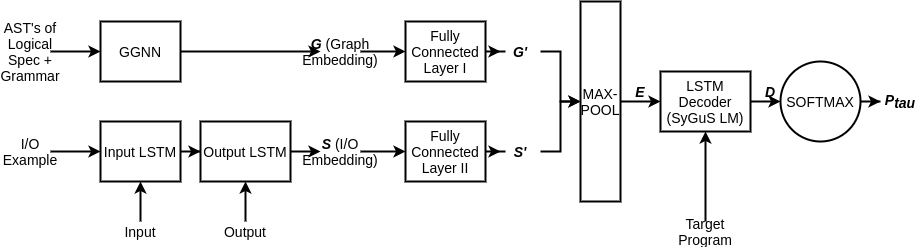
\includegraphics[scale=0.4]{NNA1.png}
    \caption{Proposed Neural Network Architecture. The dimensions of all the hidden state vectors $\mathcal{G}$,                 $\mathcal{S}$, $\mathcal{G^{'}}$, $\mathcal{S^{'}}$, $\mathcal{E}$, $\mathcal{D}$, is 128-by-1 and size of $P_\tau$ is       equal to the size of Vocabulary. The Encoder gives output as $\mathcal{E}$, which is then passed to the Decoder LSTM to     get the program token probabilities $P_\tau$}
    \label{fig:nna}
\end{figure*}

\subsubsection{Neural Network Architectures}
This section explains different architectures to be used in this work.

\paragraph{RNN}
Recurrent Neural Networks or RNN (Fig. \ref{fig:rnn}) are generally applied to sequential data. Given a Sequence of input ($x_1$,....,$x_T$), an RNN computes the sequence of outputs ($y_1$,....,$y_T$) by iterating the following equation:
\begin{align*}
    h_t = sigmoid(U{x_t}, V{h_{t-1}})\\
    y_t = W{h_t}
\end{align*}
where $h_t$ represents hidden state of RNN.
\begin{figure*}
    \centering
    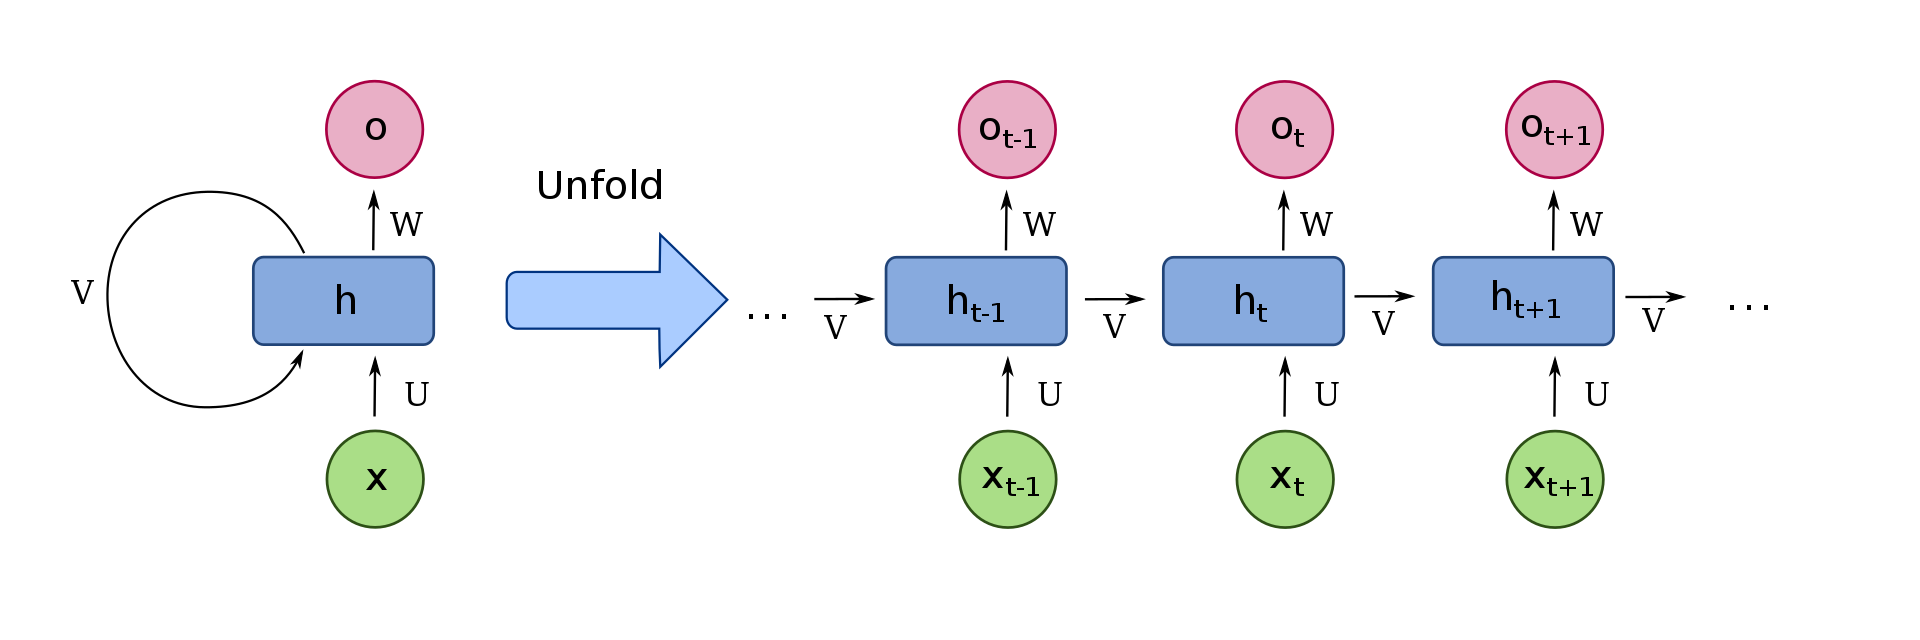
\includegraphics[scale=0.2]{rnnunfolding.png}
    \caption{Recurrent Neural Network (RNN) Cell $x_t$: input vector, $h_t$: hidden state vector, $o_t$: output vector, W, U and V: parameter matrices}
    \label{fig:rnn}
\end{figure*}

The RNN can easily encode sequences to sequences whenever the alignment between the inputs the outputs is known ahead of time (i.e both having same lengths). However, the application of an RNN to problems whose input and the output sequences have different lengths is not very clear. Cho et al. \cite{cho2014learning} uses one RNN to encode input to a fixed-size vector and uses another RNN to generate output sequence from the fixed-size vector. Theoretically this approach should work but it is seen practically that it fails to recall long-term dependencies (\cite{bengio1994learning}, \cite{hochreiter2001gradient}). However, LSTM's \cite{hochreiter1997long} are able to capture the long term temporal dependency in the sequence.

\paragraph{Gated Recurrent Unit}
Gated Recurrent Unit (Fig \ref{fig:gru}) or GRU cell is an RNN cell with gates for controlling the amount of information to be retained from the past. Initially, for t=0, the output vector is $h_{0}=0$. \footnote{https://en.wikipedia.org/wiki/Gated\_recurrent\_unit}
%Variables:
%{\displaystyle $x_{t}$}$x_{t}$: input vector
%{\displaystyle $h_{t}$}$h_{t}$: output vector
%{\displaystyle {$\hat {h}}_{t}}{\displaystyle {\hat {h}}_{t}}: candidate activation vector
%{\displaystyle z_{t}}z_{t}: update gate vector
%{\displaystyle r_{t}}r_{t}: reset gate vector
%{\displaystyle W}W, {\displaystyle U}U and {\displaystyle b}b: parameter matrices and vector

%Activation functions:
%{\displaystyle \sigma _{g}}\sigma _{g}: The original is a sigmoid function.
%{\displaystyle \phi _{h}}\phi _{h}: The original is a hyperbolic tangent.
\begin{figure*}
    \centering
    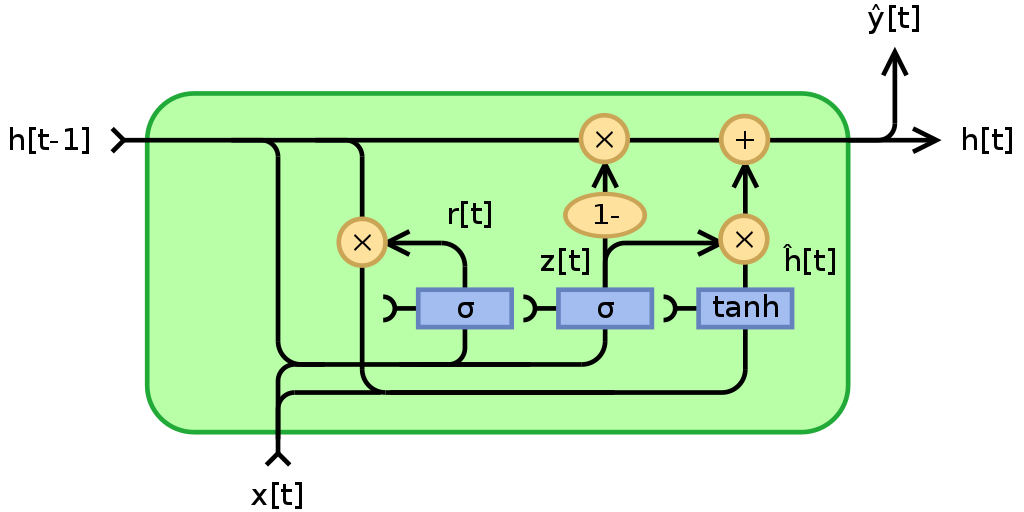
\includegraphics[scale=0.2]{gru.png}
    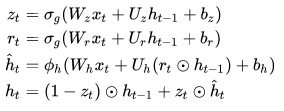
\includegraphics[scale=0.4]{grueqn.png}
    \caption{Gated Recurrent Unit (GRU) Cell, Propagation Model ($x_t$: input vector, $h_t$: hidden state, $\hat{h_t}$: candidate activation vector, $z_t$: update gate vector, $r_t$: reset gate vector, W, U and b: parameter matrices and vector, $\sigma_g$: sigmoid, $\phi_h$: tanh}
    \label{fig:gru}
\end{figure*}

\paragraph{LSTM}
LSTM estimates the conditional probability $p(y_1,...,y_{T^{'}} | x_1,...,x_T)$ where ($x_1,...,x_T$) is an input sequence and $y_1,...,y_{T^{'}}$ is an output sequence whose length $T^{'}$ may be different from the length of input sequence. The LSTM computes this conditional probability by first by learning a fixed-dimensional representation v of the input sequence ($x_1,...,x_T$) which is the last hidden state of the LSTM. This representation vector v is then passed to another LSTM, as an initial hidden state, that serves as a Language Model (trained over the Grammar of required output language) to compute the probability of $y_1,...,y_{T^{'}}$ \begin{align*}
    p(y_1,..,y_{T^{'}} | x_1,..,x_T) = \\ \Pi_{t=1}^{T^{'}}p(y_t|v,y_1,..,y_{t-1})
\end{align*}
Where $p(y_t | v,y_1,...,y_{t-1})$ distribution is represented with a softmax operation over the vocabulary (unique tokens in the output grammar G). The first LSTM is the Encoder part of a Seq2Seq architecture while the second one is the Decoder part. Fig. \ref{fig:lstm} shows a schematic diagram of an LSTM Cell.

\begin{figure*}
    \centering
    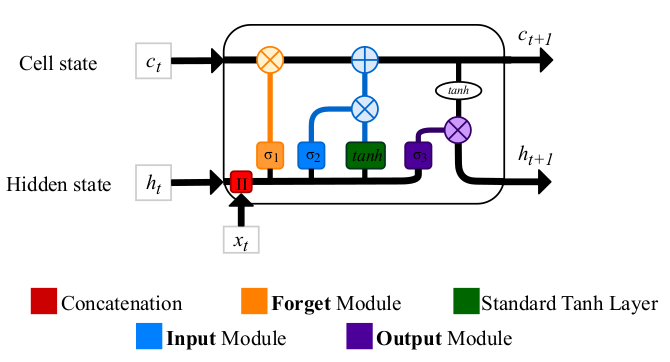
\includegraphics[scale=0.4]{lstm.png}
    \caption{Long-Short Term Memory (LSTM) Cell}
    \label{fig:lstm}
\end{figure*}

\paragraph{Gated Graph Neural Network (GGNN)}
\label{gnn}
We use Gated Graph Neural Network (Fig. \ref{fig:ggnn}) (Li et al., 2015)\cite{li2015gated} for representing specifications. This part gives a brief understanding of how GGNN works. Let G = (V, E, X) be a graph with V being set of vertices, E = ($E_1$, $E_2$, ..., $E_k$) be the set of directed edges where k is the number of edge types, and X is the feature set of nodes. In our case k=2 types of edges viz. intrinsic and extrinsic depending upon whether it is connecting nodes internal to grammar or logical spec or is it connecting the grammar and logical spec graphs together. Each vertex v $\in$ V is annotated with feature vector $x^{(v)}$ $\in$ $R^d$ representing the features of node (e.g. embedding of node label).

\begin{figure*}
    \centering
    \includegraphics[scale=0.5]{GGNN.png}
    \caption{(a) An Example Gated Graph Neural Network (GGNN), (b) Message Passing}
    \label{fig:ggnn}
\end{figure*}

Each of the node is associated with a state embedding vector ${h^t}^{(v)}$ at time step t, initialized with node feature vector $x^{(v)}$. The sizes of State vector and feature vector are kept same ($R^d$). Information is propagated among each nodes of the graph by Message Passing. Each node v receives messages of type k from its neighbours u, where each message is computed from its current state vector as ${m^t}_{k}^{(u)}$ = $f_{k}({h^t}^{(u)})$. Here, $f_{k}$ can be an arbitrary function which we choose to be a Linear Layer that transforms the state vector with a dxd weight matrix W as $f_{k}({h^t}^{(u)})$ $=$ ($W \cdot {h^t}^{(u)}$). All the state vectors are updated at same time by aggregating all the messages from its neighbours as ${M^t}^{(v)}$ = g(${m^t}_{k}^{(u)}$) at time step t, where g is an aggregation function which is element-wise summation in our case. A new state vector ${h^{t+1}}^{(v)}$ for each vertex v at next time step t+1 is calculated as ${h^{t+1}}^{(v)}$ = GRU(${M^t}^{(v)}$, ${h^t}^{(v)}$), GRU is Gated Recurrent Unit (Cho et al.) \cite{chung2014empirical}. These updations are carried out for a fixed time step T and the final state vectors are used as node representation. To get a graph level representation $\mathcal{G}$ we do max pooling of final node representations as $\mathcal{G}$ = MAXPOOL(${h^t}^{(v_i)}$) for each node $v_i$.

\paragraph{Seq2Seq Architecture}
It is an Encoder-Decoder model, where the encoder encodes the input sequence (I/O Examples in our case) into an embedding vector which is passed as input to the Decoder network. The Decoder then decodes the output sequence (Sketch in our case). We use Long Short Term Memory (LSTM) both for Encoding and Decoding.

%\begin{figure*}
%    \centering
%    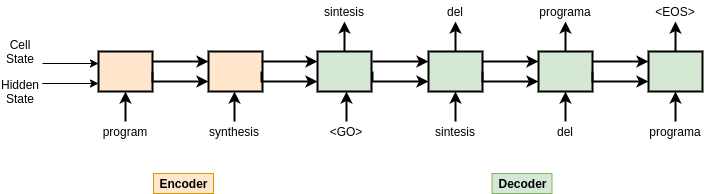
\includegraphics[scale=0.5]{seq2seq.png}
%    \caption{An Example of translating English to Spanish using Seq2Seq Architecture}
%    \label{fig:seq}
%\end{figure*}

\subsubsection{Learning Representations}
The Constraints or Semantic/ Logical Specification and the Grammar or Syntactic Specification are highly structured, which is missed when we consider them just a sequence of tokens. The structure contains important information like order of operators in the constraints or derivations of the grammar. However, it may fail to see the semantic similarity of syntactically different constraints. Consider the following three constraints - 

(1) ($\implies$ (= (mod x 2) 0) (= (+ (div1 x) (div1 x)) x))
    
(2) (not ($\implies$ (= (mod x 2) 0) (= (+ (div1 x) (div1 x)) x)))

(3) ($\implies$ (True) ($\implies$ (= (mod x 2) 0) (= (+ (div1 x) (div1 x)) x)))

Assume same grammar G for all three constraints. Constraints are said to deliver the semantics of the function to be synthesized but still due to its symbolic nature, constraints (1) and (2) are considered syntactically much more similar than constraints (1) and (3) despite the fact that (1) and (3) are essentially asking for same function i.e division by 2.

While I/O examples can encode concrete functional behaviour of intended function to be synthesized. For e.g. {(4, 2), (10, 5)} I/O pairs clearly concludes that (1) and (3) are semantically equivalent. But I/O examples suffers from insufficient path coverage. And even for covered paths, it requires huge dataset to achieve generalization, leading to expensive training procedure.

Therefore we aim to benefit from both kinds of specifications viz. SMT and I/O examples. For this we present a novel approach for learning representations of both SMT spec and I/O spec. This idea is based on Learning Blended, Precise Semantic Program Embeddings by Wang et al. \cite{wang2019learning}

\paragraph{Encoder: Learning Representations for Logical spec and given Grammar}
In order to retain the structural properties of constraints and grammar we construct GGNN for the underlying AST's. Each node of the GGNN is a GRU cell and each edge is a feed forward network. It is trained and the final graph embedding $\mathcal{G}$ are obtained as explained in \ref{gnn}. Our architecture for learning representations for syntactic and semantic specification is similar to the one used by Xujie Si \cite{si2018learning} which joins the graphs of logical specification and the grammar together as one graph. In addition, we extend it for General Track of SyGuS Competition.
%Therefore we use Gated Graph Neural Network to learn the representation

\paragraph{Encoder: Learning Representations for I/O spec}
We use an \textbf{input LSTM encoder} and an \textbf{output LSTM encoder} as described in deepsynth \cite{polgreen2020counterexample}. Each argument of the input(I) of an I/O example is fed to the input LSTM. The final hidden state of the input LSTM encoder becomes the initial hidden state of the output LSTM encoder and the output (O) is fed as input to it. The final hidden state of the output LSTM is the learned representation of one I/O example. Embeddings for all the I/O examples of a program are aggregated together to get the final I/O embedding $\mathcal{S}$.

\paragraph{Aggregating $\mathcal{G}$ and $\mathcal{S}$}
Finally we learn a combined representation for both logical spec and the I/O spec by aggregating the two embeddings $\mathcal{G}$ and $\mathcal{S}$ by first passing them through a fully connected neural network and then performing max pooling operation on them. We denote this final embedding by $\mathcal{E}$. %We pass this embedding $\mathcal{E}$ through a Softmax layer to get the token probability distribution $P_\tau$ where $\tau$ denotes the set of tokens.

\subsubsection{Decoder: Neural Network for Synthesizing sketches}
%The Token probabilities $P_\tau$ 
Final embedding $\mathcal{E}$ from the Encoder is then passed to an LSTM decoder, which is a Language Model trained over SyGuS Grammar, to produce final hidden representation $\mathcal{D}$. We pass this embedding $\mathcal{D}$ through a Softmax layer to get the token probability distribution $P_\tau$ where $\tau$ denotes the set of tokens. The Decoder at each time step $t$ predicts the next most probable token $\tau_i$. $\tau_i$ is given as input to the LSTM decoder for the next time step. At each time step token with highest probability is generated. This is called Greedy Decoding technique. Greedy Decoding is an irreversible process i.e. if a wrong token is generated then it will lead to a wrong sketch, there's no way to backtrack. Therefore, we use Beam Search Decoding, which searches for $\mathcal{K}$ most probable tokens at each time step and generates $\mathcal{K}$ most likely sketches.

\subsubsection{Solving Sketches and Training the Neural Network}
The sketches generated by the Decoder is given to a Solver which finally generates $\mathcal{K}$ complete programs $P_{\mathcal{K}}$. These are then compared with the true program $\mathcal{P}$ and cross-entropy loss is calculated as follows:
$$\mathcal{L} = -\sum_{i=1}^{d}\mathcal{P}_i.log(P_{\mathcal{K}_i})$$

where $P_\mathcal{K}$ and $\mathcal{P}$ are 128 dimensional vectors denoting the output programs and the ground truth programs. $\mathcal{P}_i$ and $P_{\mathcal{K}_i}$ are the $i^{th}$ dimension value of $\mathcal{P}$ and $P_\mathcal{K}$ respectively. We train our network by the method of \textit{teacher forcing}, in which the target sequence is fed to the Decoder directly during the training and used to compute the next token. The final program $P_{final}$ obtained by minimizing the loss $\mathcal{L}$, is our solution program.

%Instructions for Ravi:
%Add the NN proposal here as explained in Skype.
%Add the RL report in appendix.tex of this report
